\subsection{Use Case with Dynamic Reputation Management}
\label{sec:use_case_with_drm}

Now if we take a look at the use case outlined in Section \ref{subsec:use_case} with the Dynamic Reputation Management solution, we can prevent the behavior of user 1 from affecting the other users in the system. Figure \ref{image:airline_reservation_with_drm} shows the use case with the reputation management solution embedded. In this scenario, the bad reputation of user 1 doesn't affect user 2. We have tracked the reputation of user 1 and therefore prevent user 1 from reserving the seat. This then allows the seat to be available for user 2 to reserve and purchase.

\begin{figure}
\centering
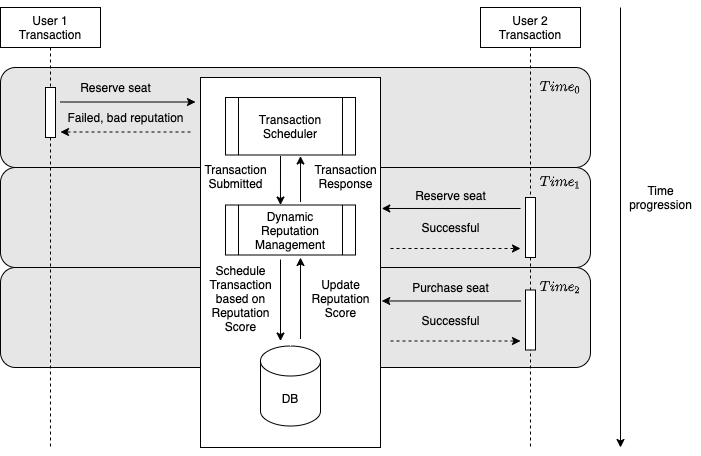
\includegraphics[scale=0.50]{images/AirlineReservation_w_DRM.png}
\caption{Use Case with Dynamic Reputation Management}
\label{image:airline_reservation_with_drm}
\end{figure}